\section{Solutions aux exigences de client}
     \begin{frame}{Solutions aux exigences de client}{}
        \begin{itemize}
          \item<1-> Analyse lexicale couplée avec l'analyse syntaxique
          \item<2-> Génération d’un arbre syntaxique abstrait couplée avec une analyse sémantique.
          \item<3-> Génération du code intermédiaire.
          \item<4-> Compilation du code intermédiaire en objet machine.
        \end{itemize}
     \end{frame}
   %%%%
   \subsection{Schématisation de la compilation}
      \begin{frame}{Solutions aux exigences de client}{Schématisation de la compilation}
        \begin{block}{Schématisation de la compilation}
          \begin{figure}[!h]
            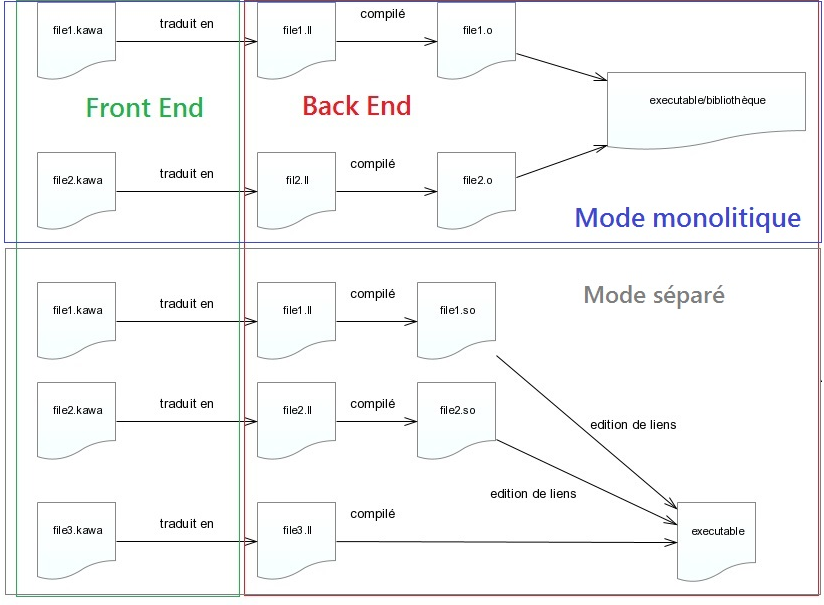
\includegraphics[width=8cm]{../res/presentation/fig2.png}
            \caption{Processus de compilation}
            \label{processus_de_compilation}
          \end{figure}
        \end{block}
      \end{frame}
    %%%%
   \subsection{Outils de réalisation Front End}
      \begin{frame}{Solutions aux exigences de client}{Outils de réalisation Front End}
        \begin{block}{Outils de réalisation Front End}
          \begin{itemize}
            \item<1-> Langage de programmation: C++
            \begin{itemize}
              \item<2-> Contrainte imposée par le client motivé par la disponibilité d'une API LLVM permettant la production du code intermédiaire LLVM.
            \end{itemize}
            \item<3-> Langage Cible: code IR LLVM
            \begin{itemize}
              \item<4-> Le code IR LLVM est un langage à part entière capable de réaliser les exigences du client. 
            \end{itemize}
          \end{itemize}
        \end{block}
      \end{frame}
    %%%%
    \subsection{Outils de réalisation Back End}
      \begin{frame}{Solutions aux exigences de client}{Outils de réalisation Back End}
        \begin{block}{Outils de réalisation Back End}
          \begin{itemize}
            \item<1-> Outils de compilation de code intermédiaire
            \begin{itemize}
              \item<2-> opt: Optimisation de code LLVM
              \item<3-> llc: Compilateur de code IR
              \item<4-> lld: Éditeur de lien
              \item<5-> clang: Compilateur compatible code IR.
            \end{itemize}
            
          \end{itemize}
        \end{block}
      \end{frame}
       %%%%
    \subsection{Extension du document d'architecture}
      \begin{frame}{Solutions aux exigences de client}{Extension du document d'architecture}
        \begin{block}{Extension du document d'architecture}
          \begin{itemize}
            \item<1-> Des détails de la réalisation seront à résoudre lors du processus de développement.
            \item<2-> Impossible de fournir une architecture garantissant à 100\% la réalisation du projet. 
            \item<3-> Les découvertes faites seront rajoutées au document d’architecture logiciel.
          \end{itemize}
        \end{block}
      \end{frame}
  
  %%%%%%%%%%%%%%%